% !TeX program = lualatex
% !TeX root = luaking.tex
% !TeX encoding = UTF-8
% !TeX spellcheck = cs_CZ
%---------------------------------------------------------------------------------------------------
% file fey1ch45.tex
%---------------------------------------------------------------------------------------------------
%=========================== Kapitola: Ilustrace termodynamiky ====================================
\setchaptertoc
\chapter{Ilustrace termodynamiky}\label{fyz:IchapXLV}
  \section{Vnitřní energie}\label{fyz:IchapXLVsecI}
    Termodynamika je poměrně těžká a složitá ve svých aplikacích a bylo by nepřiměřené, kdybychom se
    v tomto kurzu pouštěli při těchto aplikacích příliš do hloubky. je velmi důležitá pro inženýry a
    chemiky, Zájemci se o ní mohou poučit ve fyzikální chemii nebo inženýrské termodynamice.
    Existuje mnoho dobrých příruček, jako např. Zemanskyho „Teplo a termodynamika“, 
    \begin{itemize}[noitemsep]
      \item Úvod do fyziky v řešených příkladech - (\cite{Havrankova1995}).
      \item Fyzika - Vysokoškolská učebnice obecné fyziky - (\cite{Halliday2001}).
      \item Úvod do fyziky v řešených příkladech - (\cite{Havrankova1995}).
      \item Fundamentals of Thermodynamic - (\cite{Borgnakke2012}).
    \end{itemize}
    v nichž se o termodynamice dozvíme hodně. 

    Termodynamika je tak složitá, protože jednu věc můžeme popsat mnoha způsoby. Chceme-li popsat
    chování plynu, můžeme vycházet z toho, že tlak závisí na teplotě a na objemu nebo z toho, že
    objem závisí na teplotě a tlaku. Zajímáme-li se o vnitřní energii \(U\), můžeme vycházet z toho,
    že závisí na teplotě a objemu, ale proměnné si můžeme zvolit i jinak a pak můžeme vycházet z
    toho, že závisí na teplotě a tlaku nebo na tlaku a objemu apod. V poslední kapitole jsme mluvili
    i jiné funkci teploty a objemu, kterou jsme nazývali entropie a můžeme sestrojit ještě mnoho
    jiných funkcí těchto proměnných: například \(U - TS\) je funkcí teploty a objemu. Máme tedy
    mnoho různých veličin, jež mohou být funkcemi rozmanitých kombinací proměnných. Abychom
    nekomplikovali situaci, budeme v této kapitole uvažovat jako nezávisle proměnné teplotu a objem.
    Chemici používají jako nezávislé proměnné teplotu a tlak, protože se snáze měří a ovládají v
    chemických experimentech, ale my budeme v celé kapitole používat teplotu a objem až na jednu
    výjimku, když budeme vysvětlovat, jak se uskutečňuje transformace na chemický systém proměnných.
    
    Budeme tedy uvažovat jen jeden systém nezávislých proměnných: teplotu a objem. Dalším
    omezením bude to, že se budeme zajímat jen o dvě závislé funkce: o vnitřní energii a tlak. O
    ostatních funkcích nebudeme mluvit, neboť je lze odvodit z uvedených dvou funkcí. I přes tato
    omezení je termodynamika stále dost obtížný předmět, i když už ne tolik.

    Nejdříve si zopakujeme něco z matematiky. Je-li veličina funkcí dvou proměnných, musíme být
    opatrnější při jejím derivování než v případě jedné proměnné. Co rozumíme derivací tlaku podle
    teploty? Změny tlaku provázející teplotní změny částečně závisí na tom, co se děje s objemem,
    když se mění teplota \(T\). Dříve než pojem derivace podle \(T\) nabude přesný smysl, musíme
    říci něco o změnách objemu. Například se můžeme ptát, jaká je rychlost změny \(p\) vzhledem k
    \(T\), je-li \(V\) konstantní. Tato rychlost je právě obyčejnou derivací, kterou jsme zvyklí
    psát jako \(\diff{p}{T}\). Abychom si připomněli skutečnost, že \(p\) kromě toho, že závisí na
    \(T\), závisí i na jiné proměnné a tuto proměnnou považujeme za konstantu \(V\), obvykle
    používáme speciální symbol \(\diffp pT[]\). Na upozornění, že druhá proměnná se nemění,
    používáme nejen symbol \(\partial\), ale i index označující proměnnou, kterou považujeme za
    konstantu, tedy píšeme \(\diffp pV[V]\). Máme-li jen dvě proměnné, je takové
    označení zbytečné, ale pomůže nám lépe se orientovat v džungli parciálních derivací
    termodynamiky.

    Předpokládejme, že funkce \(f(x, y)\) závisí na dvou nezávislých proměnných \(x\) a \(y\). Pod
    \(\diffp fx[y]\) rozumíme obyčejnou derivací získanou obvyklým způsobem, považujeme-li \(y\) za
    konstantu:
    \begin{align*}
      \left(\pder{f}{x}\right)_y = \lim_{\Delta x \rightarrow0} 
                                   \dfrac{f(x+\Delta x,y) - f(x,y)}{\Delta x}   \\
      \shortintertext{Podobně definujeme}
      \left(\pder{f}{y}\right)_x = \lim_{\Delta y \rightarrow0} 
                                   \dfrac{f(x,y +\Delta y) - f(x,y)}{\Delta y}  
    \end{align*}

    Například, je-li \(f(x, y) =x^2 + yx\), pak \(\diffp fx[y] = 2x + y\) a \(\diffp fy[x] = x\).
    Tuto myšlenku můžeme zobecnit i na vyšší derivace: \(\diffp[2]f/y\) nebo \(\diffp f{x,y}\).
    Poslední symbol znamená, že nejdříve derivujeme \(f\) podle \(x\) a přitom považujeme \(y\) za
    konstantu a pak derivujeme výsledek podle \(y\) a považujeme \(x\) za konstantu. Skutečné pořadí
    derivování není podstatné: \(\diffp f{x,y} = \diffp f{y,x}\).

    Budeme potřebovat vypočítat změnu \(\Delta f\) funkce \(f(x, y)\), když \(x\) se mění na \(x +
    \Delta x\) a \(y\) se mění na \(y + \Delta y\). Předpokládejme, že \(\Delta x\) a \(\Delta y\)
    jsou infinitezimálně malé
    \begin{align}
      \Delta f &= f(x+\Delta x, y+\Delta y) =                                \nonumber  \\
               &= \underbrace{f(x+Δx,y+Δy)−f(x,y+Δy)}_{\Delta x\diffp fx[y]} \nonumber  \\
               &+ \underbrace{f(x,y+Δy)−f(x,y)}_{\Delta y\diffp fy[x]}       \nonumber  \\
               &= \Delta x\diffp fx[y] + \Delta y\diffp fy[x]                \label{fyz:eq779}
    \end{align}
    Poslední rovnice je základním vztahem, jenž vyjadřuje \(\Delta f\) pomocí \(\Delta x\) a
    \(\Delta y\).

    Jako příklad použití tohoto vztahu vypočítejme změnu vnitřní energie \(U(T, V)\) při změně
    teploty z \(T\) na \(T + \Delta T\) a změně objemu z \(V\) na \(V+ \Delta V\). Použijeme-li
    rovnici (\ref{fyz:eq779}), můžeme psát
    \begin{equation}\label{fyz:eq780}
      ΔU=ΔT\diffp UT[V]+ΔV\diffp UV[T].
    \end{equation}
    V předcházející kapitole jsme našli jiné vyjádření změny \(\Delta U\) vnitřní energie při dodání
    tepla \(\Delta Q\) plynu
    \begin{equation}\label{fyz:eq783}
      ΔU=ΔQ−pΔV.
    \end{equation}

    \begin{figure}[ht!] %\ref{fyz:fig463}
      \centering
      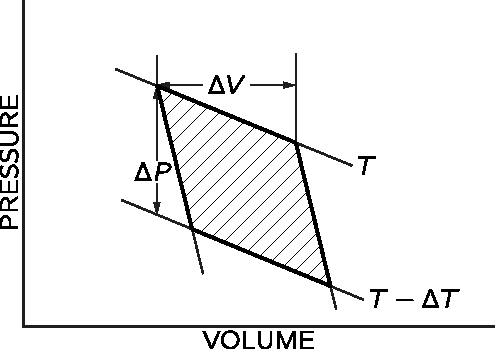
\includegraphics[width=0.7\linewidth]{fyz_fig463.pdf}
      \caption{\(p-V\) diagram Carnotova cyklu. Křivky označené \(T\) a \(\Delta T\) jsou izotermy,
               strmější křivky jsou adiabaty. A \(V\) je objemová změna plynu, jemuž bylo při
               konstantní teplotě dodáno teplo \(\Delta Q\). \(\Delta p\) je změna tlaku plynu, když
               se při konstantním objemu změnila teplota z hodnoty \(T\) na hodnotu \(T - \Delta
               T\). (\cite[s.~615]{Feynman01})}
      \label{fyz:fig463}
    \end{figure}

    Porovnání rovnic (\ref{fyz:eq780}) a (\ref{fyz:eq783}) by nás mohlo přivést na myšlenku, že \(p
    = \diffp UV[T]\), jenže taková představa není správná. Abychom získali správný vztah, nejdříve
    předpokládejme, že plynu dodáme teplo \(\Delta Q\), zatímco objem zůstane stejný, tedy \(\Delta
    V= 0\). Když \(\Delta  V = 0\), rovnice (\ref{fyz:eq783}) nám říká, že \(\Delta U=\Delta Q\) a
    z rovnice (\ref{fyz:eq780}) dostaneme \(ΔU=\diffp UT[V]ΔT\), takže \(\diffp UT[V]=ΔQ/ΔT\). Poměr
    \(ΔQ/ΔT\) představuje množství tepla, které musíme dodat látce, aby se při konstantním objemu
    změnila její teplota o jeden stupeň, nazývá se \textbf{měrná tepelná kapacita při konstantním
    objemu} a označuje se symbolem \(C_V\). Takovým způsobem jsme ukázali, že
    \begin{equation}\label{fyz:eq783}
      \diffp UT[V] = C_V.
    \end{equation}

    Nyní dodejme plynu opět množství tepla \(\Delta Q\), ale při stálé teplotě \(T\) a objem ať se
    změní o \(\Delta V\). V takovém případě je analýza složitější, ale \(\Delta U\) můžeme počítat s
    použitím Carnotových argumentů a k tomu nám poslouží Camotův cyklus, o němž jsme mluvili v
    předcházející kapitole.

    Diagram tlak - objem pro Carnotův cyklus je znázoměn na obr. \ref{fyz:fig463}. Už dříve jsme
    ukázali, že celkové množství práce konané plynem při vratném cyklu je rovno \(ΔQ(ΔT/T)\), kde
    \(ΔQ\) je množství tepelné energie dodané plynu při izotermické expanzi při teplotě \(T\) z
    objemu \(V\) na \(V+ΔV\) a \(T−ΔT\) je výsledná teplota, které plyn dosáhne při adiabatické
    expanzi v druhé části cyklu. Nyní ukážeme, že tato vykonaná práce je rovna vyšrafované ploše na
    obr. \ref{fyz:fig463}. Práce plynu je rovna ve všech případech \(\int p\dd{V}\) a je kladná,
    když se plyn rozpíná a záporná, když je stlačován. Nakreslíme-li \(p\) v závislosti na \(V\),
    pak změny \(p\) a vvystihuje křivka, která každé hodnotě \(V\) přiřazuje určitou hodnotu \(p\).
    Mění-li se objem z jedné hodnoty na druhou, práce konaná plynem, tedy integrál \(\int p\dd{V}\),
    je plocha pod křivkou spojující počáteční a konečnou hodnotu \(V\). Aplikujeme-li tuto
    myšlenku na Camotův cyklus a dáme pozor na znaménko práce plynu, opravdu zjistíme, že čistá
    práce plynu je právě vyšrafovaná plocha na obr. \ref{fyz:fig463}.

    Nyní vyjádříme vyšrafovanou plochu geometricky. Cyklus znázorněný na obr. \ref{fyz:fig463} se
    liší od cyklu z předcházející kapitoly v tom, že nyní \(\Delta T\) a \(\Delta Q\) jsou
    infinitezimálně malé. Pracujeme mezi adiabatickými a izotermickými čarami, které jsou velmi
    těsně u sebe, a proto se obrazec, nakreslený na obr. \ref{fyz:fig463} silnými čarami bude blížit
    rovnoběžníku, když \(\Delta T\) a \(\Delta Q Q\) půjdou k nule. Plocha tohoto rovnoběžníku je
    právě \(ΔVΔP\), kde \(ΔV\) je změna objemu plynu při dodání energie \(ΔQ\) pñ konstantní teplotě
    a \(Δp\) je změna tlaku při změně teploty o \(ΔT\) při stálém objemu. To, že je vyšrafovaná
    plocha na obr. \ref{fyz:fig463} rovna \(ΔVΔP\), snadno nahlédneme, uvážíme-li, že taková plocha
    je rovna ploše ohraničené přerušovanou čárou na obr. \ref{fyz:fig464}, která se od pravoúhelníku
    ohraničeného \(Δp\) a \(ΔV\) liší jen přidáním a odebráním stejných trojúhelníkových ploch.

    \begin{figure}[ht!] %\ref{fyz:fig464}
      \centering
      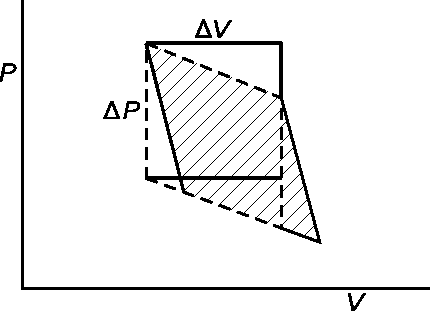
\includegraphics[width=0.7\linewidth]{fyz_fig464.pdf}
      \caption{Vyšrafovaná plocha = plocha ohraničená přerušovanými čárami = plocha pravoúhelníku =
               \(\Delta p \Delta V\) (\cite[s.~616]{Feynman01})}
      \label{fyz:fig464}
    \end{figure}

    Shrňme naše dosavadní úvahy:
    \begin{mdframed}[style=mdmathdef]  
      \begin{definition}\label{fyz:def001}
        Práce konaná plynem = vyšrafovaná plocha = \(ΔVΔP=ΔQ\left(\dfrac{ΔT}{T}\right)\) nebo
        \begin{align*}
          \dfrac{ΔT}{T}
            &\cdot\text{(teplo potřebné ke změně \(V\) 
              o \(\Delta V\))}_{T=\text{konst}}              \\
            &=                                               \\
          \Delta V
            &\cdot\text{(změna \(p\) při změně \(T\) 
              o \(\Delta T\))}_{V=\text{konst}}               \\
          \shortintertext{nebo} 
          \dfrac{1}{\Delta V}
            &\cdot\text{(teplo potřebné ke změně \(V\) 
              o \(\Delta V\))}_T                              \\
            &= T\diffp PT[V].
        \end{align*}
      \end{definition}
    \end{mdframed}
    Vztahy v definici (\ref{fyz:def001}) vyjadřují to podstatné, co vyplývá z Carnotových úvah.
    Celou termodynamiku můžeme odvodit z (\ref{fyz:def001}) a prvního zákona, který je vyjádřen
    rovnicí (\ref{fyz:eq783}). Rovnice v (\ref{fyz:def001}) představují vlastně druhý zákom, i když
    ten byl původně odvozen Carnotem v trochu jiném tvaru, protože Carnot nepoužil naší definici
    teploty.

    Nyní můžeme přistoupit kvýpočtu \(\diffp UT[V]\). O kolik se změní vnitřní energie \(U\),
    změníme-li objem o \(\Delta  V\) ? Vnitřní energie se mění, protože je dodáváno teplo a protože
    se koná práce. Dodané teplo je podle vztahu (\ref{fyz:def001}) rovna
    \begin{equation*}
      ΔQ=T\diffp pT[V] ΔV,
    \end{equation*}
    a s látkou konaná práce je rovna \(-p\Delta V\). Proto změna vnitřní energie \(\Delta U\) se
    skládá ze dvou částí
    \begin{equation}\label{fyz:eq784}
      ΔU=T\diffp pT[V]ΔV−pΔV.
    \end{equation}
    Dělíme-li obě strany rovnice \(\Delta V\), najdeme rychlost změny \(U\) v závislosti na \(V\)
    při konstantní teplotě \(T\)
    \begin{equation}\label{fyz:eq785}
      \diffp UV[T] = T\diffp pT[V]−p.
    \end{equation}
    V naší termodynamice, kde \(T\) a \(V\) jsou jediné proměnné a \(p\) a \(U\) jsou jediné funkce,
    představují rovnice (\label{fyz:eq783}) a (\ref{fyz:eq785}) základní vztahy, z nichž můžeme
    získat všechny výsledky.

  \section{Aplikace}\label{fyz:IchapXLVsecII}
    Nyní se zamyslíme nad významem rovnice (\ref{fyz:eq785}) a všimneme si, proč dává odpověď na
    otázky, které jsme položili v předcházející kapitole. Uvažovali jsme následující problém: v
    kinetické teorii je zřejmé, že růst teploty vede k růstu tlaku v důsledku nárazů atomů na píst.
    Ze stejného fyzikálního důvodu je při zpětném pohybu pístu z plynu odváděno teplo a abychom
    udrželi konstantní teplotu, musíme teplo dodat. Při expanzi se plyn ochlazuje a při ohřívání
    plynu tlak roste. Mezi těmito dvěma jevy musí existovat určitá souvislost a tato souvislost je
    explicitně dána rovnicí (\ref{fyz:eq785}). Kdybychom zachovali objem a zvýšili teplotu, tlak by
    vzrostl rychlostí \(\diffp pT[V]\). S touto skutečností souvisí i následující. Zvětšíme-li
    objem, plyn se ochladí, pokud nedodáme určité teplo k udržování konstantní teploty a veličina
    \(\diffp UV[T]\) nám říká, kolik tepla je třeba k udržení teploty dodat. Rovnice
    (\ref{fyz:eq785}) vyjadřuje základní vztah mezi těmito dvěma jevy a to je věc, kterou jsme
    slíbili zjistit, když jsme se dostali až k termodynamickým zákonům. Aniž bychom znali vnitřní
    mechanismus plynu a za pomoci jediného poznatku, že nelze sestrojit perpetuum mobile druhého
    druhu, jsme odvodili vztah mezi množstvím tepla potřebným k udržení konstantní teploty při
    rozpínání plynu a změnou tlaku při ohřátí plynu!

    Nyní, když jsme si poradili s plynem uvažujme pásek gumy. Když takový pásek napínáme,
    zjišťujeme, že jeho teplota klesá a když ho ohříváme, vidíme, že se smršťuje. Jak vypadá
    rovnice, která by poskytovala pro pásek gumy stejný vztah, jako dává rovnice (\ref{fyz:eq783})
    pro plyn? V případě pásku gumy bude situace asi taková: když dodáme teplo \(ΔQ\), změní se
    vnitřní energie o \(ΔU\) a vykoná se určitá práce. Jediný rozdíl je v tom, že práce konaná
    páskem gumy je \(-FΔL\) místo \(pΔV\), přičemž \(F\) je síla působící na pásek a \(L\) je délka
    pásku. Síla \(F\) je funkcí teploty a délky pásku. Nahradíme-li \(pΔV\) v rovnici
    (\ref{fyz:eq783}) výrazem \(-FΔL\), dostaneme
    \begin{equation}\label{fyz:eq786}
      ΔU=ΔQ+FΔL.      
    \end{equation}
    Porovnáním rovnic (\ref{fyz:eq783}) a (\ref{fyz:eq786}) zjistíme, že rovnici pro gumový pásek
    získáme pouhou záměnou písmen. Zaměníme-li \(L\) za \(V\) a \(-F\) za \(p\), můžeme naše úvahy o
    Carnotově cyklu aplikovat na pásek gumy. Pak okamžitě zjistíme, že například teplo \(ΔQ\),
    potřebné ke změně délky o \(ΔL\), je dáno analogem defince (\ref{fyz:def001}):  \(ΔQ = -T\diffp
    FT[L]ΔL\). Udržujeme-li konstantní délku pásku a ohříváme ho, umožní nám tato rovnice vypočítat
    vzrůst síly vyjádřený pomocí tepla potřebného k udržování konstantní teploty při malém natažení
    pásku. Vidíme tedy, že stejné rovnice můžeme aplikovat na plyn i na pásek gumy. Když můžeme psát
    \(ΔU=ΔQ+AΔB\), kde \(A\) a \(B\) představují různé veličiny, sílu a délku, tlak a objem apod.,
    pak výsledky pro plyn získáme tak, že místo \(A\) a \(B\) dosadíme \(p\) a \(V\). Jako příklad
    uvažujme rozdíl elektrických potenciálů nebo napětí \(E\) baterie a náboj \(ΔZ\), který prochází
    baterií. Víme, že práce konaná vratnou elektrickou baterií, takovou jako je např. akumulátor, je
    rovna \(EΔZ\). (Neuvažujeme-li ve vyjádření pro práci člen \(pΔV\), předpokládáme, že baterie má
    konstantní objem.) Podívejme se, co nám řekne termodynamika o činnosti baterie. Dosadíme-li
    hodnotu \(E\) místo \(p\) a hodnotu \(Z\) místo \(V\), dostaneme z rovnice (\ref{fyz:eq784})
    \begin{equation}\label{fyz:eq787}
      \dfrac{ΔU}{ΔZ}=T\diffp ET[Z]−E.
    \end{equation}
    Rovnice (\ref{fyz:eq787}) říká, když baterií prochází náboj \(ΔZ\), změní se vnitřní energie
    \(U\). Proč se \(\tfrac{ΔU}{ΔZ}\) nerovná prostě napětí \(E\) baterie? Důvod je ten, že skutečná
    baterie se zahřívá, prochází-li jí proud. Vnitřní energie baterie se mění jednak proto, že
    baterie koná určitou práci ve vnějším obvodu a jednak proto, že se baterie ohřeje. Pozoruhodné
    je to, že tu druhou část změny vnitřní energie můžeme opět určit pomocí změny napětí baterie s
    teplotou. Mimochodem, když baterií prochází náboj, dochází k chemické reakci a rovnice
    (\ref{fyz:eq787}) poskytuje elegantní způsob měření energie potřebné k uskutečnění chemické
    reakce. Potřebujeme jen zhotovit baterii využívající takovou reakci, změřit napětí a změřit, jak
    se mění napětí s teplotou, když z baterie neodebíráme náboj!

  
  \section{Clasiova-Clapeyronova rovnice}\label{fyz:IchapXLVsecIII}
  
    \begin{figure}[ht!] %\ref{fyz:fig465}
      \centering
      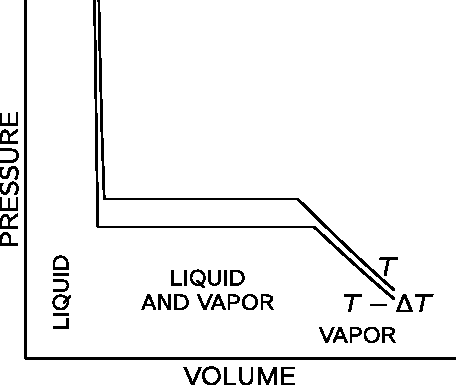
\includegraphics[width=0.7\linewidth]{fyz_fig465.pdf}
      \caption{ 
              (\cite[s.~707]{Feynman01})}
      \label{fyz:fig465}
    \end{figure}

    \begin{figure}[ht!] %\ref{fyz:fig466}
      \centering
      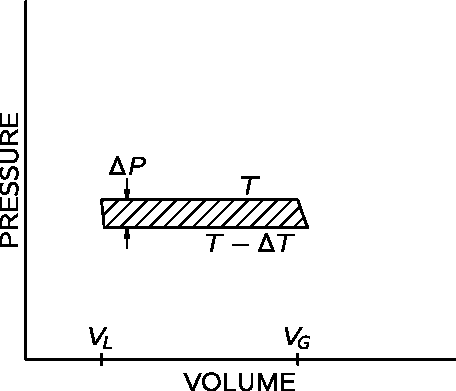
\includegraphics[width=0.7\linewidth]{fyz_fig466.pdf}
      \caption{ 
              (\cite[s.~707]{Feynman01})}
      \label{fyz:fig466}
    \end{figure}
  \section{Příklady a cvičení}\label{fyz:IchapXLVsecIV}
    \subsection{Výhřevnost paliva}\label{fyz:IchapXLVsecIVssecI}
      Výhřevnost \(H\) [\si{\joule\per\kg}] je vlastnost paliva, která udává, kolik energie se
      uvolní úplným spálením jedné jednotky (obvykle \SI{1}{\kg}). Proti spalnému teplu není v
      hodnotě zahrnuto měrné skupenské teplo páry, obsažené ve spalinách. Předpokládá se, že její
      teplo je nevyužitelné a uniká v plynném stavu se spalinami.

      Výhřevnost je dána vztahem
      \begin{equation*}
        H=\dfrac{Q}{m}
      \end{equation*}
      kde \(Q\) je uvolněné teplo a \(m\) je hmotnost paliva. 

      %-Palivo potřebné k letu----------------------------------------
      % !TeX spellcheck = cs_CZ
\begin{mdframed}[style=mdexam]
  \begin{example}\label{FYZ:exam028}
    \emph{Proudové letadlo má čtyři motry, z nich každý vyvíjí tahovu sílu \SI{20}{\kN}. Jaká je
    hmotnost paliva potřebného k letu o délce \SI{5000}{\km}? Výhřevnost paliva je
    \SI{45}{\mega\joule\per\kg}, učinnost motorů \SI{25}{\percent}.(\cite[s.~32]{Bartuska1997})}  

    {\centering
    \captionsetup{type=figure}
    \luafigure[1]{fyz_fig0933.pdf}
    \captionof{figure}{Řez proudovým motorem (\cite[s.~500]{Borgnakke2012})
    \label{fyz:fig0933}}
    \par} 
    
    \textbf{Řešení:}\newline 
    Při práci proudových motorů se část enerige, která se uvolní spálením paliva, spotřebuje na
    vykonání práce. Účinnost motorů je určena vztahem:
    \begin{equation*}
      \eta = \dfrac{W}{Q_1},
    \end{equation*}
    kde \(W = nFs\) je práce, kterou vykonají motory letadla, a \(Q_1 = m_1H\) teplo, které se
    uvolní při letu letadla spálením paliva o hmotnosti \(m_1\) a výhřevnosti \(H\). Užitím těchto
    vztahů dostáváme
    \begin{equation*}
     W = \eta Q_1 = \eta m_1H = nFs \quad\rightarrow\quad m_1 = \dfrac{nFs}{\eta H}.
    \end{equation*}
    Čísleně 
    \begin{align*}
       m_1 &= \dfrac{4\cdot\SI{20}{\kN}\cdot\SI{5000}{\km}}
                    {\num{0.25}\cdot\SI{45}{\mega\joule\per\kg}}                                  \\
       m_1 &= \dfrac{4\cdot\num{2e4}\cdot\num{5e6}}{\num{0.25}\cdot\num{45e6}}\cdot
              \dfrac{\si{\kg\m\per\square\s}\cdot\si{\m}}{\si{\kg\square\m\per\square\s\per\kg}}  \\
       m_1 &\approx \SI{35.6e3}{\kg} \approx \SI{36}{\tonne}        
     \end{align*}
     K letu letadla na dráze \SI{5000}{\km} je zapotřebí palivo o hmotnosti \SI{36}{\tonne}.
  \end{example} 
\end{mdframed}
      %---------------------------------------------------------------
      %-Množství petroleje na ohřátí vody-----------------------------
      % !TeX spellcheck = cs_CZ
\begin{mdframed}[style=mdexam]
  \begin{example}\label{FYZ:exam029}
    \emph{Určete hmotnost petroleje, který spotřebuje petrolejový vařič k zahřátí vody o hmotnosti
    \SI{3}{\kg} z \SI{10}{\degreeCelsius} na \SI{100}{\degreeCelsius}. Účinnost vařiče
    \SI{34}{\percent}, výhřevnost petroleje je \SI{44}{\mega\joule\per\kg} a měrná kapacita vody
    \SI{4180}{\joule\per\kg\per\kelvin}. (\cite[s.~31]{Bartuska1997})}
    
    {\centering
    \captionsetup{type=figure}
    \luafigure[1]{fyz_fig934.png}
    \captionof{figure}{Abychom si v terénu dokázali teplé jídlo připravit, neobejdeme se bez vody a
    bez spolehlivého vařiče a paliva.
    \label{fyz:fig934}}
    \par} 
    
    \textbf{Řešení:}\newline 
    Při ohřívání vody petrolejovým vařičem se jen část tepla, které se uvolní při spalování
    petroleje, spotřebuje na ohřátí vody. Účinnost vařiče je určena vztahem:
    \begin{equation*}
      \eta = \dfrac{Q}{Q_1},
    \end{equation*}
    kde \(Q = mc(t_2 - t_1)\) je teplo, které přijme voda  hmotnosti \(m\) při ohřátí z teploty
    \(t_1\) na teplotu \(t_2\), a \(Q=m_1H\) teplo uvolněné spálením petroleje o hmotnosti \(m_1\)
    a výhřevnosti \(H\). Užitím těchto vztahů dostáváme
    dostáváme
    \begin{align*}
     Q = \eta Q_1 = \eta m_1H &= mc(t_2-t_1) \;\rightarrow  \\
                               m_1 &= \dfrac{mc(t_2-t_1)}{\eta H}.
    \end{align*}
    Čísleně 
    \begin{align*}
       m_1 &= \dfrac{\SI{3}{\kg}\cdot\SI{4180}{\joule\per\kg\per\kelvin}\cdot\SI{90}{\kelvin}}
                    {\num{0.34}\cdot\SI{44}{\mega\joule\per\kg}}                                  \\
       m_1 &= \dfrac{3\cdot4180\cdot90}{\num{0.34}\cdot\num{44e6}}\cdot
              \dfrac{\si{\kg}\cdot\si{\joule\per\kg\per\kelvin}\cdot\si{\kelvin}}
                    {\si{\J\per\kg}}                                                              \\
       m_1 &\approx \SI{75}{\g}    
     \end{align*}
     Na zahřátí vody o hmotnosti \SI{3}{\kg} z \SI{10}{\degreeCelsius} na \SI{100}{\degreeCelsius}
     na petrolejovém vařiči je zapotřebí \SI{75}{\g} petroleje.
  \end{example} 
\end{mdframed}
      %---------------------------------------------------------------
      %-Množství střelného prachu v nábojnici-------------------------
      % !TeX spellcheck = cs_CZ
\begin{mdframed}[style=mdexam]
  \begin{example}\label{FYZ:exam030}
    \emph{Určete hmotnost střelného prachu v nábojnici, jestliže střela má hmotnost \SI{20}{\g} a
    při výstřelu získá rychlost \SI{700}{\m\per\s}. Výhřevnost střelného prachu je
    \SI{3.79}{\mega\joule\per\kg} a účinnost zbraně je \SI{28}{\percent}.
    (\cite[s.~31]{Bartuska1997})}
    
    \textbf{Řešení:}\newline 
    Při výstřelu se část energie, která se uvolní při spálení střelného prachu přemění na kineticku
    energii střely. Účinnost zbraně je určena vztahem:
    \begin{equation*}
      \eta = \dfrac{E_k}{Q_1},
    \end{equation*}
    kde \(E_k = \frac{1}{2}mv^2\) je kinetická energie střeli a \(Q_1 = m_1H\) je celkové teplo,
    které se při výstřelu uvolní spálením střelného prachu o hmotnosti \(m_1\) a výhřevnosti \(H\).
    Užitím těchto vztahů dostáváme dostáváme
    \begin{equation*}
     E_k = \eta Q_1 = \eta m_1H = \frac{1}{2}mv^2 \;\rightarrow\; m_1 = \dfrac{mv^2}{2\eta H}.
    \end{equation*}
    Čísleně 
    \begin{align*}
       m_1 &= \dfrac{\SI{20}{\g}\cdot(\SI{700}{\m\per\s})^2}
                    {2\cdot\num{0.28}\cdot\SI{3.79}{\mega\joule\per\kg}}                          \\
       m_1 &= \dfrac{\num{0.02}\cdot700^2}{\num{0.56}\cdot\num{3.79e6}}\cdot
              \dfrac{\si{\kg}\cdot\si{\square\m\per\square\s}}
                    {\si{\kg\square\m\per\square\s\per\kg}}                                       \\
       m_1 &\approx \SI{4.6}{\g}    
     \end{align*}
     V nábojnici je střelný prach o hmotnosti \SI{4.6}{\g}.
  \end{example} 
\end{mdframed}
      %---------------------------------------------------------------
      %-Automobil-----------------------------------------------------
      % !TeX spellcheck = cs_CZ
\begin{mdframed}[style=mdexam]
  \begin{example}\label{FYZ:exam030}
    \emph{Automobil, jehož motor má výkon \SI{40}{\kW}  a účinnost \SI{28}{\percent}, se pohybuje
    rychlostí \SI{120}{\km\per\hour}. Jakou dráhu může urazit, jestliže zásoba paliva v nádrži je
    \SI{20}{\litre}? Výhřevnost paliva je \SI{46}{\mega\joule\per\kg}, jeho hustota
    \SI{750}{\kg\per\cubic\m}. (\cite[s.~33]{Bartuska1997})}
    
    \textbf{Řešení:}\newline 
    Účinnost automobilového motoru je určena vztahem:
    \begin{equation*}
      \eta = \dfrac{W}{Q_1},
    \end{equation*}
    kde \(W\) je práce, kterou vykoná motor automobilu při jízdě na dráze \(s\) a \(Q_1 = m_1H\)
    teplo, které se při jízdě po této dráze uvolní spálením paliva o hmotnosti \(m_1\) a výhřevnost
    \(H\). Pro práci \(W\) proto platí: 
    \begin{equation*}
     W = \eta Q_1 = \eta m_1H = \eta\varrho VH.
    \end{equation*}
    Výkon automobilového motoru při jízdě na dráze \(s = vt\) je \(P=\dfrac{W}{t}\). Odtud pro práci
    \(W\) dostáváme
    \begin{equation*}
      W = Pt = P\dfrac{s}{t}. 
    \end{equation*}
    Z předchozích rovnic pak vyplývá
    \begin{equation*}
      P\dfrac{s}{t} = \eta\varrho VH \;\rightarrow\; s = \dfrac{\eta\varrho VHv}{P}
    \end{equation*}
    číselně
    \begin{align*}
       s  &=  \dfrac{\num{0.33}\cdot750\cdot\num{30e-3}\cdot\num{46e6}\cdot\num{33.3}}{\num{40e3}}
              \cdot                   
           =  \dfrac{\si{\kg}\cdot\si{\square\m\per\square\s}}
                    {\si{\kg\square\m\per\square\s\per\kg}}                                       \\
       m_1 &\approx \SI{4.6}{\g}    
     \end{align*}
     V nábojnici je střelný prach o hmotnosti \SI{4.6}{\g}.
  \end{example} 
\end{mdframed}
      %---------------------------------------------------------------
    
    \subsection{Kalorimetrická rovnice}\label{fyz:IchapXLVsecIVssecII}
      %-Hmotnost vaříí vody-------------------------------------------
      % !TeX spellcheck = cs_CZ
\begin{mdframed}[style=mdexam]
  \begin{example}\label{FYZ:exam032}
    \emph{Určete hmotnost vařící vody, kterou je třeba přilít do vody o hmotnosti \qty{5}{\kg} a
    teplotě \qty{9}{\degreeCelsius}, aby výsledná teplota vody byla \qty{30}{\degreeCelsius}.
    Předpokládejme, že tepelná výměna nastala jen mezi teplejší a studenější vodou. 
     (\cite[s.~33]{Bartuska1997})}
    
    \textbf{Řešení:}\newline 
    Teplo, které odevzdá vařicí voda, se rovná teplu, které přijme studenejší voda. Platí proto
    \begin{equation*}
      m_Hc(t_2 - t) = m_Sc(t-t_1), \;\rightarrow\; m_H = \dfrac{(t_2 - t)}{(t-t_1)}\cdot m_S.
    \end{equation*}
    číselně
    \begin{align*}
      m_H &= \dfrac{(\qty{30}{\degreeCelsius}  -  \qty{9}{\degreeCelsius})}
                  {(\qty{100}{\degreeCelsius} - \qty{30}{\degreeCelsius})}\cdot\qty{5}{\kg}.         \\
      m_H &= \qty{1.5}{\kg}
    \end{align*}
    Do studenejší vody je třeba přilít vařicí vodu o hmotnosti \qty{1.5}{\kg}.  
  \end{example} 
\end{mdframed}
      %--------------------------------------------------------------- 
      %-Teplota pece--------------------------------------------------
      % !TeX spellcheck = cs_CZ
\begin{mdframed}[style=mdexam]
  \begin{example}\label{FYZ:exam033}
    \emph{Do vody o hmotnosti \SI{800}{\g} a teplotě \SI{12}{\degreeCelsius} byla ponořena platinová
    koule o hmotnosti \SI{150}{\g}, která byla předtím ponechána v žáru pece. Po dosažení
    rovnovážného stavu byla výsledná teplota soustavy \SI{19}{\degreeCelsius}. Určete teplotu pece.
    Měrná tepelná kapacita platiny je \SI{133}{\joule\per\kg\per\kelvin}. Předpokládejme, že tepelná
    výměna nastala jen mezi platinovou koulí a vodou. (\cite[s.~34]{Bartuska1997})}
    
    \textbf{Řešení:}\newline 
    Podle kalorimetrické rovnice se teplo, které odevzdá platinová koule, rovná teplu, které přijme
    voda a výsledná teplota soustavy \(t=\SI{19}{\degreeCelsius}\). Platí proto
    \begin{equation*}
      m_Pc_P(t_2 - t) = m_Vc_V(t-t_1), \;\rightarrow\; t_2 = \dfrac{m_Vc_V(t - t_1)}{m_Pc_P} + t_1.
    \end{equation*}
    číselně
    \begin{align*}
      t_2 &= \dfrac{\SI{800}{\g}\cdot\SI{4180}{\joule\per\kg\per\kelvin}          %
              \cdot(\SI{ 19}{\degreeCelsius} - \SI{12}{\degreeCelsius})}
                   {\SI{150}{\g}\cdot\SI{133}{\joule\per\kg\per\kelvin}}          \\
      t_2 &=\SI{1192}{\degreeCelsius}
    \end{align*}
    Teplota pece je asi \SI{1200}{\degreeCelsius}. Při ponoření zahřáté platinové koule se část vody
    odpaří. Teplo potřebné k tomuto odpaření jsme neuvažovali.  
  \end{example} 
\end{mdframed}
      %---------------------------------------------------------------  
    
    \todo[inline]{Kapitola fey1ch45 je zcela prázdná, pouze obrázky} 
%---------------------------------------------------------------------------------------------------